Per la navigazione del robot, in particolare del robot \textit{Kid}, � stato utilizzato un approccio misto che utilizza sussunzione e metodologia a campi di potenziale.

\subsection{Campi di potenziale}
	I campi previsti dall'architettura sono i seguenti:
	\begin{itemize}
	    \item Wander
	    \item Avoid
	    \item Move To Goal
	\end{itemize}
	Le forze esercitate dai campi di potenziale hanno per convenzione intensit� nell'intervallo $[0,1]$. \\
	 \\
	Il campo Wander, che permette l'esplorazione dell'ambiente, applica al robot una forza costante in avanti rispetto al suo orientamento. 
	Con cadenza costante, il campo genera una forza con un orientamento rispetto al sistema di riferimento del robot tra i -90� e i +90� in maniera casuale. %TODO sicuro?
	Il vettore generato ha la massima intensit� possibile.
	% Plot del campo Avoid
	\begin{figure}[h!]
		\centering
		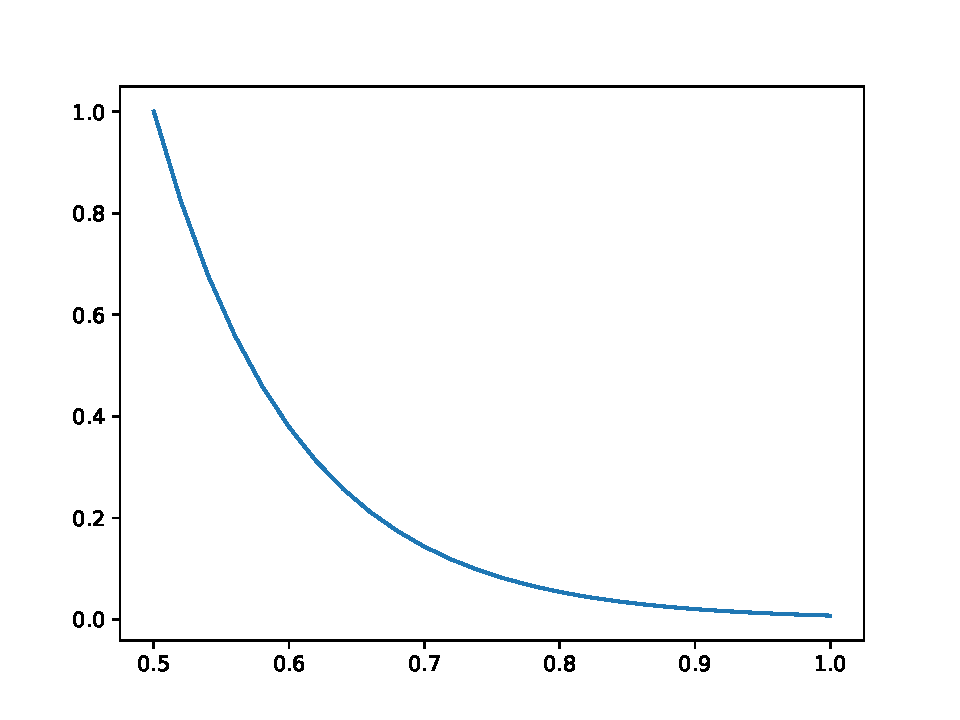
\includegraphics[width=0.7\textwidth]{images/repulsionplot.pdf}
		\caption{Plot della funzione del campo Avoid. Sull'asse delle ascisse troviamo la distanza dall'ostacolo, su quello delle ordinate l'intensit� del campo repulsivo.}
		\label{fig:repulsion_plot}
	\end{figure}
	\newpage
	Il campo Avoid permette la \textit{Obstacle Avoidance}. Ogni ostacolo genera un campo repulsivo con un profilo di ampiezza esponenziale. In particolare, l'intensit� della forza generata dal campo segue la funzione:
	\begin{center}
		$avoid(d) = b^{-c (d-D_S)} $
	\end{center}
	dove $d$ � la distanza del robot dall'oggetto, $b$ e $c$ sono fattori che determinano il comportamento della curva e $D_S$ � una distanza di sicurezza, fissata a priori.
	Il campo viene percepito solo quando la distanza dall'oggetto � di almeno 1 metro.
	La Figura~\ref{fig:repulsion_plot} evidenzia come la forza esercitata dal campo abbia intensit� massima quando l'oggetto si trova ad una distanza vicina quella di sicurezza e minima al limite della percezione del campo.\\ \\
	%Plot del campo Move to Goal
	\begin{figure}[h!]
		\centering
		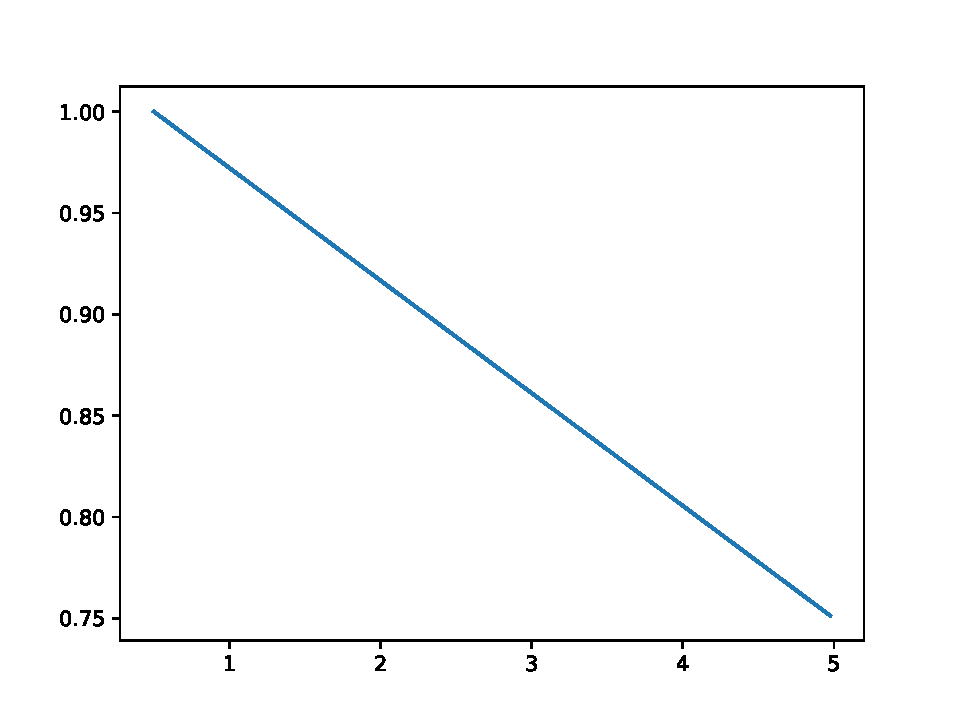
\includegraphics[width=0.7\textwidth]{images/attractionplot.pdf}
		\caption{Plot della funzione del campo Move to Goal. Sull'asse delle ascisse troviamo la distanza dall'ostacolo, su quello delle ordinate l'intensit� del campo attrattivo.}
		\label{fig:attraction_plot}
	\end{figure}

	Il campo Move to Goal permette al robot di raggiungere un punto di interesse che, nel caso in esame, � il colore a cui avvicinarsi. Il punto di interesse (POI) genera un campo attrattivo di intensit� lineare sulla distanza dal robot. Questo segue la seguente funzione:
	\begin{center}
		$attract(d) = \frac{1-F_{min}}{D_S-D_A} (d-D_S)+1$
	\end{center}
	dove $F_{min}$ � la minima intensit� garantita dal campo mentre $D_S$ e $D_A$ sono rispettivamente la distanza di sicurezza e la minima distanza di percezione del campo.
	Il campo viene percepito solo quando l'oggetto si trova ad una distanza affidabile, ovvero tale per cui il riconoscimento dello stesso ha una certa affidabilit�. Nel caso in questione, in cui il punto di interesse viene riconosciuto da una telecamera RGB-D, la rilevazione � affidabile quando l'oggetto si trova ad una distanza di al pi� 5 metri.
	La Figura~\ref{fig:attraction_plot} mostra come la forza esercitata dal campo abbia intensit� massima quando l'oggetto si trova vicino al POI, mentre a distanza massima di percezione garantisca comunque un'intensit� abbastanza elevata, permettendo al robot di raggiungere il punto di interesse pi� o meno velocemente.

\subsection{Orientamento}
	Il sistema di coordinate utilizzato � robocentrico, ovvero ogni punto rilevante (ostacoli, punto di interesse) nello spazio � individuato da coordinate ottenute dalle misurazioni dei sensori che il robot utilizza.\newline Questo sistema rende molto facile l'utilizzo dei campi di potenziale per l'individuazione di un vettore che determini il movimento del robot.
	Un problema che sorge dall'utilizzo di questo sistema � quello di gestire punti di cui non si hanno pi� rilevazioni dai sensori. Nel caso specifico del robot Kid, se esso non ha pi� visibilit� del POI che cerca di raggiungere, ad esempio perch� si � dovuto girare per evitare un'ostacolo, dovrebbe comunque poter stimare la posizione dell'oggetto.
	Per fare ci� � necessario memorizzare lo spostamento e la rotazione effettuati dal sistema di riferimento rispetto all'ultima volta in cui tale oggetto � stato rilevato.
	Ottenere questi dati � possibile grazie all'utilizzo dell'interfaccia RosAria per la gestione della mobilit� del robot. Il nodo ROS RosAria pubblica sul topic \texttt {/RosAria/pose} le informazioni sulla posizione e sull'orientamento del robot. I messaggi pubblicati sul topic utilizzano un sistema di coordinate mondocentrico, in cui orientamento e origine coincidono con l'orientamento e la posizione del robot al momento dell'avvio del nodo RosAria.
	Per calcolare lo spostamento e la rotazione effettuata dal robot, basta memorizzare le informazioni pubblicate sul topic al momento dell'ultima rilevazione del punto di interesse e le informazioni "attuali" fornite da RosAria.
	Il vettore di traslazione e la matrice di rotazione sono calcolati come segue:
	\begin{center}
		$t = (p_s - p_c) R_s$
	\end{center}
	
	\begin{center}
		$R = 
		\begin{bmatrix}
			\cos(\theta) & -\sin(\theta) \\
			\sin(\theta) & \cos(\theta)
		\end{bmatrix}$
	\end{center}
	dove $p_s$ e $p_c$ sono  rispettivamente la posizione al momento dell'ultima rilevazione dell'oggetto di interesse e la corrente. $R_s$ � la matrice di rotazione al momento dell'ultima rilevazione del POI e $\theta$ � l'ampiezza dell'angolo di cui � ruotato il robot rispetto all'ultima rilevazione.\\
	\newpage
	Il punto di interesse, una volta fuori dal campo visivo del robot, viene calcolato come segue %TODO
	\begin{center}
		$POI_c = (POI_s + t) R$
	\end{center}
	dove $POI_s$ � la posizione del punto di interesse al momento dell'ultima rilevazione.
\subsection{Movimento} %TODO ??
	Lo schema motorio � costituito da un'unica funzione \texttt{move}, che decide il movimento del robot in base alla forza complessiva esercitata dai campi di potenziale. La coordinata x della forza determina la rotazione del robot, mentre la y determina l'intensit� del movimento in avanti.
	La velocit� lineare e quella angolare, data la forza $F$, sono cos� rispettivamente  calcolate:
	\begin{center}
		$v = \frac{F_y}{4}$
	\end{center}
	\begin{center}
		$\omega = \frac{F_x}{2}$
	\end{center}
	In questo modo la velocit� lineare massima raggiunta � di $0.25$ $m/s$ mentre quella angolare assume un valore massimo di $1.57$ $rad/s$ ($90�/s$).
	